% This file: 			Prelim. draft for Heckman to see progress
% Contributors: 		Pietro Biroli, Daniela Del Boca, Linor Kiknadze, 
%					Yu Kyung Koh, Sylvi Kuperman, Sidharth Moktan, 
%					Chiara Pronzato, Nirali Trevedi, Anna Ziff
% Original date: 		10/10/16
% Project: 			Reggio Evaluation

\documentclass[12pt]{article}
\usepackage[top=1in, bottom=1in, left=1in, right=1in]{geometry}
\parindent 22pt

\usepackage{adjustbox}
\usepackage{amsmath}
\usepackage{amssymb}
\usepackage{array}
\usepackage{booktabs}
\usepackage{datetime}
\usepackage{fancyhdr}
\usepackage{float}
\usepackage{graphicx}
\usepackage[colorlinks=true,linkcolor=blue,urlcolor=blue,anchorcolor=blue,citecolor=blue]{hyperref}
\usepackage{lscape}
\usepackage{multirow}
\usepackage{natbib}
\usepackage{setspace}
\usepackage{tabularx}
\usepackage[colorinlistoftodos,linecolor=black]{todonotes}
\usepackage{appendix}
\usepackage{pgffor}
\usepackage{caption} 
\usepackage{threeparttable}
\captionsetup[table]{skip=3pt}

\settimeformat{hhmmsstime}

\newcolumntype{L}[1]{>{\raggedright\arraybackslash}p{#1}}
\newcolumntype{C}[1]{>{\centering\arraybackslash}p{#1}}
\newcolumntype{R}[1]{>{\raggedleft\arraybackslash}p{#1}}


\usepackage{sectsty}
\sectionfont{\fontsize{14}{14}\selectfont}
\subsectionfont{\fontsize{13}{13}\selectfont}

\begin{document}

\title{\normalsize \textbf{Evaluation of the Reggio Approach} \\ \normalsize Draft}
\author{\normalsize Reggio Team}
\date{\normalsize Original version: October 3, 2016 \\ Current version: \today}
\maketitle

\doublespacing

This draft presents (i) a brief description of the data, (ii) a simple analysis comparing individuals who attended the Reggio Emilia municipal schools to individuals in Reggio Emilia who did not attend any preschool, and (iii) a discussion of selection into preschool on observed characteristics. 

\section{Data}
\label{sec:data}

The sample is a subset of the individuals in Reggio Emilia, Parma, and Padova who were born in the year ranges of the five cohorts.  These individuals were collected from the population registries in each of the cities. The sample was then restricted to those individuals living in the same city in which they were raised. All cohorts except the youngest one comprised only individuals who are Italian citizens. In contrast, the youngest cohort includes an oversampling of immigrant children.\footnote{In the adult cohorts there was no immigrant who was born in the any of the three cities and still lived there. In the adolescent cohort, the number was immigrant born was extremely small.} The sample from Reggio Emilia, across all cohorts, includes an oversampling of those who attended municipal schools, as this is the treatment group.

Of the reference sample, 7,109 individuals were randomly selected. Of these, 4,019 completed interviews, resulting in a response rate of 56.5\%. Figure~\ref{fig:sample} presents an overview of the sample highlighting those who attended a Reggio Approach preschool. Table~\ref{tab:sample} provides a detailed tabulation of the sample by city, cohort, and school type.

\begin{figure}[H]
\begin{center}
\caption{The Sample by City and Cohort}\label{fig:sample}
	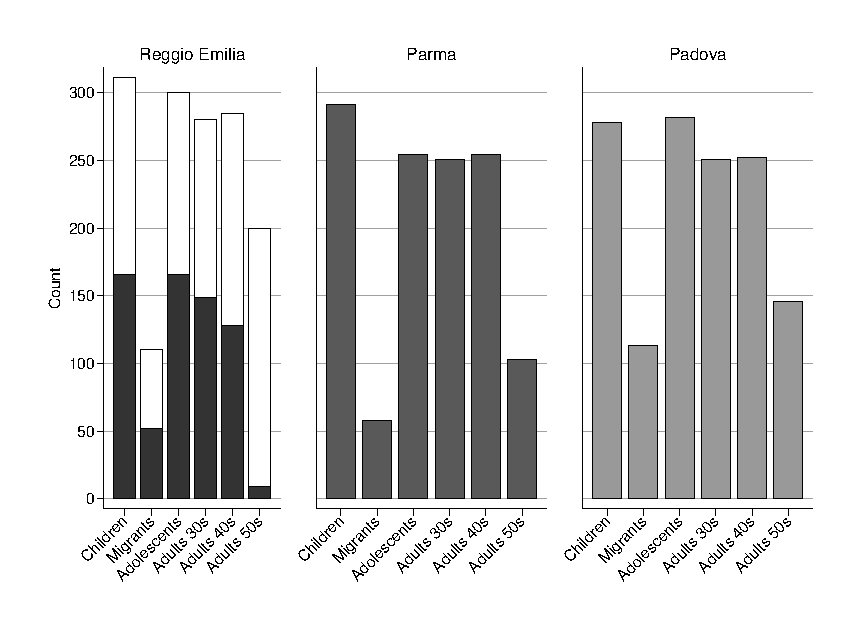
\includegraphics[width=.9\textwidth]{output/sample.eps}
\end{center}
\footnotetext{\noindent Note: This figure displays the number of individuals by cohort and city. The bars for Reggio Emilia differentiate between those who attended municipal preschool (black bars) and those who did not (white bars). Those in Reggio Emilia who attended municipal preschools are considered the treatment group.}
\end{figure}

\begin{table}[H]
\centering
\scalebox{0.7}{
\begin{threeparttable}
	\caption{The Sample by Cohort, City, and School Type}\label{tab:sample}
	\begin{tabular}{l*{15}{c}}
\toprule
            &\mc{5}{c}{Reggio Emilia: 1,471}   &     \mc{5}{c}{ Parma: 1,198}       &      \mc{5}{c}{Padova: 1,305}      \\
           \cmidrule(lr){2-6} \cmidrule(lr){7-11} \cmidrule(lr){12-16} 
      &        None&       Muni.&       State&      Relig.&       Priv.&        None&       Muni.&       State&      Relig.&       Priv.&        None&       Muni.&       State&      Relig.&       Priv.\\
\midrule
Children    &           2&         166&          45&          92&           5&           6&         154&          43&        77&           9&           2&          82&          40&         141&          12\\
Migrants    &           4&          52&          37&          14&           1&           4&          35&          10&          	3&           6&           5&          36&          47&          23&           1\\
Adolescents &           7&         166&          22&          96&           6&           4&         116&          43&     82&           6&           1&          93&          47&         131&           6\\
Adults 30    &          57&         149&          31&          40&           1&          44&          98&          51&        50&          5&       47&         35&         26&            140&    1 \\
Adults 40    &          80&         128&          17&          52&           5&         116&          52&          26&       55&          1&        75&      27 &            24&            123&   \\
Adults 50    &         147&           9&          10&          28&           2&          72&          12&           7&          11&            &        57&      11 &           2 &           68&    2 \\
\midrule
	       &         297&         670&         162&         322&          20&         246&         467&   180&    278&          27&      187&      284 &            186&        626& 22  \\
\bottomrule
\end{tabular}


\begin{tablenotes}
Note: This table shows the sample size by city, cohort, and school type. These numbers do not include individuals with an unidentified preschool type. In total, there are 45 individuals with unidentified preschool type. We separate migrants and children for clarity in this table even though they are in the same birth cohort (year of birth: 2006). None: no preschool; Muni.: municipal preschool;  State: state preschool; Relig.: religious preschool; Priv.: private preschool.
\end{tablenotes}
\end{threeparttable}
}
\end{table}

The structure of the cohorts allows us to study the effects of the Reggio Approach at different points throughout the life cycle. The youngest cohort of children were interviewed when they entered primary school, the adolescent cohort when they ended compulsory schooling, and the adult cohorts capture different points of adulthood to measure key outcomes such as engagement in the labor market, health, and family decisions. This cohort structure also allows us to evaluate the Reggio Approach compared to the alternative early childhood experiences over time.

Separate questionnaires were administered to the children, adolescents, and adults. as well as to the caregivers of the children and adolescents. The questionnaires include items about early childhood experiences, family structure, education, interaction with non-Italians (or with Italians in the case of the migrant children), and measures of cognitive and social-emotional skills. The questionnaires for adults additionally included items about occupation, income, health, and life satisfaction. 

\section{Basic Analysis}
\label{sec:methodology}

Since there are two stages of early childhood interventions, (i) ages 0-3 and (ii) ages 3-6, it is important to consider both when estimating treatment effects of either intervention on later outcomes. Table \ref{tab:cases-treat} shows the possible cases of receiving early childhood intervention in our data, where 0 indicates not attending and 1 indicates attending. For this stage, we limit the type of infant-toddler centers and preschools to municipal only. 

\begin{table}[H] \caption{Possible Cases of Treatment} \label{tab:cases-treat}

  \begin{tabular}{C{1.8cm} R{0.7cm} C{2cm} C{2cm}}
  
		& & \multicolumn{2}{c}{Preschool (Ages 3-6)} \\
		& & 0 & 1 \\ \cline{3-4}            
        								 &  & \multicolumn{1}{|c|}{} & \multicolumn{1}{c|}{} \\
        								& 0 & \multicolumn{1}{|c|}{(0,0)} & \multicolumn{1}{c|}{(0,1)} \\ 
        				ITC				&  & \multicolumn{1}{|c|}{} & \multicolumn{1}{c|}{} \\ \cline{3-4}
                        (Age 0-3)  		&  & \multicolumn{1}{|c|}{} & \multicolumn{1}{c|}{} \\
        								& 1 & \multicolumn{1}{|c|}{(1,0)} & \multicolumn{1}{c|}{(1,1)} \\ 
        								&  & \multicolumn{1}{|c|}{} & \multicolumn{1}{c|}{} \\ \cline{3-4}
  \end{tabular}
\begin{flushleft}
\tiny{{\bfseries Notes:} Sample size for the treatment group. Number of individuals in each city that attended a \textit{municipal} infant-toddler-center (ages 0-3), a \textit{municipal} preschool (ages 3-6), or both. (0,0) = did not attend any municipal school for both ages 0-3 and 3-6; (1,0) = attended a municipal school for ages 0-3 but did \textit{not} attend for ages 3-6; (0,1) = did \textit{not} attend a municipal school for ages 0-3 but did attend for ages 3-6; (1,1) = attended a municipal school for both ages 0-3 and 3-6;}
\end{flushleft}
\end{table}


\subsection{Estimating Effects of Infant-Toddler Centers}
There are two main ways of testing treatment effects of attending infant-toddler centers. First is to compare people who did not attend any municipal school for both ages 0-3 and 3-6 with people who only attended municipal infant-toddler centers for ages 0-3. This is to compare (0,0) and (1,0) in Figure \ref{tab:cases-treat}. Second is to compare people who only attended municipal preschool for ages 3-6 with people who attended both municipal infant-toddler centers and preschools. This is to compare (0,1) and (1,1) in Figure \ref{tab:cases-treat}. Formally writing, the hypotheses are:
\begin{eqnarray}
H_1: &  Y_{0,0} = Y_{1,0} \\ 
H_2: &  Y_{0,1} = Y_{1,1} 
\end{eqnarray}
where $Y_{0,0}$ is the outcome of the people who did not attend any infant-toddler center or preschool, and vice versa for other cases. 

A possible estimation strategy is to limit the sample to specific city \textit{and} specific cohort \textit{and} the comparison groups needed according to the hypothesis above. To test $H_1$, we estimate the following regression equation:
\begin{eqnarray}
Y_{i}^{c,h} & = & \alpha + \beta_{0}R_i^{ITC} + \mathbf{X_i}\gamma + \varepsilon_{i}^{c,h}, \\ \nonumber
& \forall & i \in \text{ \{People in city $c$ and cohort $h$ and in group (0,0) or (1,0)\}}
\end{eqnarray}
where $R_i^{ITC}$ is the indicator for attending municipal infant-toddler center and $\mathbf{X_i}$ is the vector of baseline variables for individual $i$. Likewise, to test $H_2$:
\begin{eqnarray}
Y_{i}^{c,h} & = & \alpha + \beta_{0}R_i^{ITC} + \mathbf{X_i}\gamma + \varepsilon_{i}^{c,h}, \\ \nonumber
& \forall & i \in \text{ \{People in city $c$ and cohort $h$ and in group (0,1) or (1,1)\}}
\end{eqnarray}

One of the caveats of this analysis is that it significantly reduces the sample size used in the analysis. In fact, the hypotheses cannot be tested using this strategy for many groups. Table \ref{tab:num-group} shows the number of people available for each group necessary for analysis using this strategy. It is easy to see that it is impossible to test $H_1$ with our data, because there are almost no people who went to municipal infant-toddler centers but did not attend any preschools (the group (1,0)). It is possible to carry out test for $H_2$ for many groups, but the number of observations for the group (1,1) is very small for the adult cohorts. 

\begin{table}[H] \caption{Number of Individuals in Each Group} \label{tab:num-group}
\scalebox{0.77}{
\begin{tabular}{l|ccccc|ccccc|ccccc}
\toprule
			& 		\multicolumn{5}{c}{\textbf{Reggio}}		& 	\multicolumn{5}{|c|}{\textbf{Parma}}	& 			\multicolumn{5}{c}{\textbf{Padova}}				\\
			& (0,0) & (1,0) & (0,1) & (1,1) & Total & (0,0) & (1,0) & (0,1) & (1,1) & Total  & (0,0) & (1,0) & (0,1) & (1,1) & Total \\ \midrule
Child		& 2 & 0 & 46 & 117 & \textbf{311} & 5 & 1 & 35 & 100 & \textbf{291} & 2 & 0 & 31 & 36 & \textbf{278} \\
Migrant		& 4 & 0	& 24 & 26 & \textbf{110} & 4 & 0 & 12 & 23 & \textbf{58} & 5 & 0 & 18 & 16 & \textbf{113} \\
Adolescent 	& 7 & 0 & 45 &	116 & \textbf{300} & 4 & 0 & 49 & 61 & \textbf{254} & 1 & 0 & 55 & 37 & \textbf{282} \\
Age-30		& 57 & 0 & \cellcolor{blue!25}95 &	\cellcolor{blue!25}53 & \textbf{280} & 43 & 0 & \cellcolor{blue!25}64 & \cellcolor{blue!25}29 & \textbf{251} & 47 & 0 & 25 & 9 & \textbf{251} \\
Age-40		& 80 & 0 & \cellcolor{blue!25}97 &	\cellcolor{blue!25}28 & \textbf{285} & 115 & 1 & 35 & 16 & \textbf{254} & 75 & 0 & 25 & 2 & \textbf{252} \\
Age-50		& 146 & 0 &	8 & 0 & \textbf{200} & 71 & 0 & 4 & 8 & \textbf{103} & 55 & 0 & 11 & 0 & \textbf{146} \\ \bottomrule
\end{tabular}}
\end{table}

In Table \ref{tab:num-group}, the groups subject to our estimation are highlighted. Since there are more outcomes for adult cohorts than younger cohorts, we first focus on analyzing the effect of infant-toddler centers on the adult cohorts. Based on the available number of individuals in each cell and the history of the foundation date of municipal asilo for each city, we decide to test $H_2$ for the following groups:
\begin{itemize}
\item Age-30 people in Reggio who did not attend any infant-toddler center and attended municipal preschool (the group (0,1)) \textbf{vs.} Age-30 people in Reggio who attended both municipal infant-toddler center and municipal preschool (the group (1,1))
\item Age-40 people in Reggio who did not attend no infant-toddler center and attended municipal preschool (the group (0,1)) \textbf{vs.} Age-40 people in Reggio who attended both municipal infant-toddler center and municipal preschool (the group (1,1))
\item Age-30 people in Parma who did not attend no infant-toddler center and attended municipal preschool (the group (0,1)) \textbf{vs.} Age-30 people in Parma who attended both municipal infant-toddler center and municipal preschool (the group (1,1))
\end{itemize}

The first two comparison above will show effects of the Reggio-Approach infant-toddler centers for each age cohort. The third comparison does not show effects of the Reggio-Approach infant-toddler centers, but shows effect of Parma infant-toddler centers for age-30 cohort. For our analysis in this draft, we only include the comparisons for Reggio individuals. 

\subsection{Estimating Effects of Preschools}
For this abbreviated analysis, we restrict to individuals from Reggio Emilia who either attended a Reggio Approach preschool or did not attend any preschool. We exclude the cohort of adults in their 50s because the Reggio Approach was not available to them.

For individual $i$ in Reggio Emilia, let $R_i^{P}$ indicate whether that individual attended a Reggio Approach preschool. We select a vector, $\bm{X}_i$, of baseline control variables with the lowest BIC to account for family background.\footnote{These variables are: gender, whether the individual took the computer-assisted (CAPI), number of siblings, an indicator if the mother's maximum education was middle school, an indicator if the father's maximum education is university, and two indicators for the number of siblings (one indicating having two or more siblings, the other indicating having three or more siblings).} For both cohorts, we estimate $\beta$ in the simple model

\begin{equation}
	Y_i = \alpha + \beta R_i^{P} + \bm{X}_i\gamma + \varepsilon_i
	\label{eq:ra-v-none}
\end{equation}

\noindent where we assume $\varepsilon_i$ to be a random disturbance. 

While this estimate is useful in gaining a basic understanding of the relation between the Reggio Approach and outcomes $Y_i$, there is a clear selection issue. That is, the choice to enroll a child in the Reggio Approach and the choice not to enroll a child in any preschool might be tied to unobservable characteristics that are also influencing the outcomes. After Section~\ref{sec:results} in which we present the estimates from Equation~\eqref{eq:ra-v-none}, we present a discussion of selection on observed characteristics.

\section{Results}
\label{sec:results}

Tables \ref{ols-E-reg} to \ref{ols-S-reg} show the OLS estimates of the effect of the Reggio Approach preschools for people in Reggio Emilia who attended Reggio Approach preschools compared to those who did not attend preschool at all. We do not include the age-50 cohort in this analysis, as the Reggio Approach did not exist for that cohort. We perform analysis using (i) no control, (ii) 6 controls selected by Bayesian Information Criterion (BIC), and (iii) the full set of controls that include baseline variables available for the adult cohorts. 

Table \ref{ols-E-reg} shows statistically significant effects of the Reggio Approach on high school grade for age-30 cohort. However, it should be noted that the high school grade measure in the data is not standardized across different schools. 


\begin{table}[H] \caption{OLS Results for Cognitive and Education, Municipal vs. None, Reggio Emilia} \label{ols-E-reg}
{
\def\sym#1{\ifmmode^{#1}\else\(^{#1}\)\fi}
\begin{tabular}{l*{6}{c}}
\toprule
            &\multicolumn{1}{c}{(1)}&\multicolumn{1}{c}{(2)}&\multicolumn{1}{c}{(3)}&\multicolumn{1}{c}{(4)}&\multicolumn{1}{c}{(5)}&\multicolumn{1}{c}{(6)}\\
            &\multicolumn{1}{c}{None30}&\multicolumn{1}{c}{BIC30}&\multicolumn{1}{c}{Full30}&\multicolumn{1}{c}{None40}&\multicolumn{1}{c}{BIC40}&\multicolumn{1}{c}{Full40}\\
\midrule
IQ Factor   &     0.00406         &      -0.220         &      -0.293         &     -0.0747         &     -0.0638         &      -0.162         \\
            &     (0.149)         &     (0.156)         &     (0.161)         &     (0.120)         &     (0.142)         &     (0.170)         \\
\addlinespace
High School Grade&       4.051\sym{*}  &       5.042\sym{*}  &       3.969         &       0.690         &       2.034         &       1.398         \\
            &     (1.961)         &     (2.130)         &     (2.401)         &     (1.395)         &     (1.618)         &     (2.232)         \\
\addlinespace
University Grade&       2.390         &      0.0387         &       0.638         &      -0.826         &      -0.222         &      -1.926         \\
            &     (2.233)         &     (2.552)         &     (2.840)         &     (2.433)         &     (2.751)         &     (5.638)         \\
\addlinespace
Graduate from High School&     -0.0424         &      0.0301         &     0.00954         &      -0.170\sym{***}&     -0.0525         &     -0.0315         \\
            &    (0.0502)         &    (0.0495)         &    (0.0577)         &    (0.0502)         &    (0.0542)         &    (0.0669)         \\
\addlinespace
Max Edu: University&      -0.120         &     -0.0673         &     -0.0744         &     -0.0188         &      0.0528         &      0.0572         \\
            &    (0.0670)         &    (0.0684)         &    (0.0716)         &    (0.0535)         &    (0.0608)         &    (0.0624)         \\
\addlinespace
Max Edu: Graduate School&     0.00671         &     0.00747         &     0.00700         &           0         &           0         &           0         \\
            &   (0.00672)         &   (0.00769)         &   (0.00744)         &         (.)         &         (.)         &         (.)         \\
\bottomrule
\end{tabular}
}

\vspace{1ex} \\
\footnotesize\raggedright{Note: This table shows the OLS estimates for attending Reggio Approach schools for people in Reggio Emilia who attended Reggio Approach preschools or no preschool at all. Column title indicates the age group and control set used in each regression corresponding to the column. ``None30'' refers to the regression with only age-30 cohort and with no control variables. ``BIC30'' refers to the regression with only age-30 cohort and with controls selected by Bayesian Information Criterion (BIC). ``Full30'' refers to the regression with only age-30 cohort and with the full set of controls. Analogous meanings applied to the age-40 cohort. Robust standard errors are reported in parentheses. Stars show statistical significance as follows. * p < 0.05, ** p < 0.01, *** p < 0.001.}
\end{table}

Table \ref{ols-W-reg} shows consistently significant positive effects of the Reggio Approach on hours worked per week. Moreover, there are significant effects on the indicator for the lowest household income category for the age-40 cohort. Note that the measures for subject labor income, including ``Monthly Wage'' presented in the table, have very few observations. Household income suffers less from the missing value problem.

\begin{table}[H] \caption{OLS Results for Employment and Income, Municipal vs. None, Reggio Emilia} \label{ols-W-reg}
\scalebox{0.92}{
{
\def\sym#1{\ifmmode^{#1}\else\(^{#1}\)\fi}
\begin{tabular}{l*{6}{c}}
\toprule
            &\multicolumn{1}{c}{(1)}&\multicolumn{1}{c}{(2)}&\multicolumn{1}{c}{(3)}&\multicolumn{1}{c}{(4)}&\multicolumn{1}{c}{(5)}&\multicolumn{1}{c}{(6)}\\
            &\multicolumn{1}{c}{None30}&\multicolumn{1}{c}{BIC30}&\multicolumn{1}{c}{Full30}&\multicolumn{1}{c}{None40}&\multicolumn{1}{c}{BIC40}&\multicolumn{1}{c}{Full40}\\
\midrule
Employed    &      0.0717         &      0.0526         &      0.0588         &      0.0652         &      0.0574\sym{*}  &    -0.00160         \\
            &    (0.0435)         &    (0.0432)         &    (0.0458)         &    (0.0348)         &    (0.0287)         &    (0.0356)         \\
\addlinespace
Self-Employed&     -0.0566         &      -0.102         &     -0.0994         &      0.0461         &      0.0126         &     0.00948         \\
            &    (0.0591)         &    (0.0631)         &    (0.0686)         &    (0.0487)         &    (0.0556)         &    (0.0763)         \\
\addlinespace
Hours Worked Per Week&       6.476\sym{**} &       6.134\sym{**} &       6.180\sym{**} &       4.736\sym{*}  &       3.648         &       4.713\sym{*}  \\
            &     (1.987)         &     (2.110)         &     (2.028)         &     (1.880)         &     (1.891)         &     (2.354)         \\
\addlinespace
Monthly Wage&      -188.4\sym{*}  &      -179.1\sym{*}  &      -192.6         &      -849.4         &     -1088.6         &       243.9         \\
            &     (74.31)         &     (88.37)         &     (118.0)         &     (699.5)         &     (758.5)         &    (1080.8)         \\
\addlinespace
Income: 5,000 Euros of Less&       0.148\sym{***}&       0.157\sym{***}&       0.173\sym{***}&     -0.0125         &    -0.00656         &     -0.0134         \\
            &    (0.0292)         &    (0.0350)         &    (0.0421)         &    (0.0125)         &   (0.00635)         &    (0.0133)         \\
\addlinespace
Income: 5,001-10,000 Euros&     -0.0284         &     -0.0220         &     -0.0278         &           0         &           0         &           0         \\
            &    (0.0254)         &    (0.0249)         &    (0.0246)         &         (.)         &         (.)         &         (.)         \\
\addlinespace
Income: 10,001-25,000 Euros&      -0.199\sym{**} &      -0.158         &      -0.217\sym{*}  &     -0.0531         &     -0.0284         &     -0.0338         \\
            &    (0.0760)         &    (0.0838)         &    (0.0897)         &    (0.0672)         &    (0.0728)         &    (0.0896)         \\
\addlinespace
Income: 25,001-50,000 Euros&      0.0741         &      0.0332         &      0.0728         &      0.0797         &      0.0464         &     -0.0259         \\
            &    (0.0780)         &    (0.0874)         &    (0.0882)         &    (0.0707)         &    (0.0754)         &    (0.0930)         \\
\addlinespace
Income: 50,001-100,000 Euros&     0.00518         &    -0.00974         &   -0.000807         &      0.0250         &      0.0365         &      0.0525         \\
            &    (0.0294)         &    (0.0306)         &    (0.0214)         &    (0.0303)         &    (0.0340)         &    (0.0317)         \\
\addlinespace
Income: 100,001-250,000 Euros&           0         &           0         &           0         &     -0.0391         &     -0.0479         &      0.0205         \\
            &         (.)         &         (.)         &         (.)         &    (0.0303)         &    (0.0299)         &    (0.0335)         \\
\addlinespace
Income: More than 250,000 Euros&           0         &           0         &           0         &           0         &           0         &           0         \\
            &         (.)         &         (.)         &         (.)         &         (.)         &         (.)         &         (.)         \\
\bottomrule
\end{tabular}
}
}
\vspace{1ex} \\
\footnotesize\raggedright{Note: This table shows the OLS estimates for attending Reggio Approach schools for people in Reggio Emilia who attended Reggio Approach preschools or no preschool at all. Column title indicates the age group and control set used in each regression corresponding to the column. ``None30'' refers to the regression with only age-30 cohort and with no control variables. ``BIC30'' refers to the regression with only age-30 cohort and with controls selected by Bayesian Information Criterion (BIC). ``Full30'' refers to the regression with only age-30 cohort and with the full set of controls. Analogous meanings applied to the age-40 cohort. Robust standard errors are reported in parentheses. Stars show statistical significance as follows. * p < 0.05, ** p < 0.01, *** p < 0.001.}
\end{table}

Table \ref{ols-L-reg} shows significant effects of the Reggio Approach on the status of being divorced for the age-30 cohort. Other results do not show any significant trend. 

\begin{table}[H] \caption{OLS Results for Living Environment, Municipal vs. None, Reggio Emilia} \label{ols-L-reg}
{
\def\sym#1{\ifmmode^{#1}\else\(^{#1}\)\fi}
\begin{tabular}{l*{6}{c}}
\toprule
            &\multicolumn{1}{c}{(1)}&\multicolumn{1}{c}{(2)}&\multicolumn{1}{c}{(3)}&\multicolumn{1}{c}{(4)}&\multicolumn{1}{c}{(5)}&\multicolumn{1}{c}{(6)}\\
            &\multicolumn{1}{c}{None30}&\multicolumn{1}{c}{BIC30}&\multicolumn{1}{c}{Full30}&\multicolumn{1}{c}{None40}&\multicolumn{1}{c}{BIC40}&\multicolumn{1}{c}{Full40}\\
\midrule
Married or Cohabitating&      0.0652         &     -0.0665         &     -0.0129         &     0.00781         &     -0.0164         &      0.0201         \\
            &    (0.0754)         &    (0.0810)         &    (0.0827)         &    (0.0618)         &    (0.0703)         &    (0.0965)         \\
\addlinespace
Divorced    &      0.0268\sym{*}  &      0.0409\sym{*}  &      0.0192         &     -0.0312         &     -0.0113         &      0.0373         \\
            &    (0.0133)         &    (0.0204)         &    (0.0130)         &    (0.0453)         &    (0.0478)         &    (0.0615)         \\
\addlinespace
Num. of Children in House&      0.0223         &      0.0172         &      0.0418         &      0.0563         &     -0.0530         &     -0.0707         \\
            &    (0.0519)         &    (0.0566)         &    (0.0603)         &    (0.0846)         &    (0.0979)         &     (0.106)         \\
\addlinespace
Own House   &    -0.00177         &      0.0830         &       0.153         &     -0.0859         &     -0.0160         &     -0.0294         \\
            &    (0.0773)         &    (0.0845)         &    (0.0899)         &    (0.0642)         &    (0.0707)         &    (0.0812)         \\
\addlinespace
Live With Parents&     -0.0613         &      -0.102         &     -0.0876         &     -0.0266         &     -0.0375         &     -0.0413         \\
            &    (0.0570)         &    (0.0531)         &    (0.0544)         &    (0.0279)         &    (0.0254)         &    (0.0297)         \\
\bottomrule
\end{tabular}
}

\vspace{1ex} \\
\footnotesize\raggedright{Note: This table shows the OLS estimates for attending Reggio Approach schools for people in Reggio Emilia who attended Reggio Approach preschools or no preschool at all. Column title indicates the age group and control set used in each regression corresponding to the column. ``None30'' refers to the regression with only age-30 cohort and with no control variables. ``BIC30'' refers to the regression with only age-30 cohort and with controls selected by Bayesian Information Criterion (BIC). ``Full30'' refers to the regression with only age-30 cohort and with the full set of controls. Analogous meanings applied to the age-40 cohort. Robust standard errors are reported in parentheses. Stars show statistical significance as follows. * p < 0.05, ** p < 0.01, *** p < 0.001.}
\end{table}

Table \ref{ols-H-reg} show that the significantly increasing effects of the Reggio Approach on numbers of days sick for the past month at the time of the interview for the age-30 cohort. Moreover, the results show the significant decreasing effects on whether the respondent has ever been suspended from school. 

\begin{table}[H] \caption{OLS Results for Health, Municipal vs. None, Reggio Emilia} \label{ols-H-reg}
{
\def\sym#1{\ifmmode^{#1}\else\(^{#1}\)\fi}
\begin{tabular}{l*{2}{c}}
\hline\hline
            &\multicolumn{1}{c}{(1)}&\multicolumn{1}{c}{(2)}\\
            &\multicolumn{1}{c}{Muni30}&\multicolumn{1}{c}{Muni40}\\
\hline
Tried Marijuana&      0.0916         &      0.0864         \\
            &    (0.0563)         &    (0.0507)         \\
[1em]
Smokes      &           0         &           0         \\
            &         (.)         &         (.)         \\
[1em]
Num. of Cigarettes Per Day&       2.431         &      -0.372         \\
            &     (1.348)         &     (1.666)         \\
[1em]
BMI         &       0.620         &      -0.220         \\
            &     (0.412)         &     (0.482)         \\
[1em]
Good Health &       0.129         &       0.126         \\
            &    (0.0775)         &     (0.103)         \\
[1em]
Num. of Days Sick Past Month&       0.285\sym{***}&      0.0400         \\
            &    (0.0848)         &    (0.0872)         \\
[1em]
Engaged in A Fight&           0         &           0         \\
            &         (.)         &         (.)         \\
[1em]
Drove Under Influence&           0         &           0         \\
            &         (.)         &         (.)         \\
[1em]
Ever Suspended from School&      -0.141\sym{**} &     -0.0159         \\
            &    (0.0521)         &    (0.0545)         \\
[1em]
Age At First Drink&      -0.518         &      -0.367         \\
            &     (1.238)         &     (1.396)         \\
\hline\hline
\multicolumn{3}{l}{\footnotesize \specialcell{\underline{Note:} This table shows the OLS estimates for people in Reggio who attended municipal preschools or none. \\                                                                         Standard errors are reported in parenthesis. Stars show statistical significance as follows: \\                                                                         * p < 0.05, ** p < 0.01, *** p < 0.001.}}\\
\end{tabular}
}

\vspace{1ex} \\
\footnotesize\raggedright{Note: This table shows the OLS estimates for attending Reggio Approach schools for people in Reggio Emilia who attended Reggio Approach preschools or no preschool at all. Column title indicates the age group and control set used in each regression corresponding to the column. ``None30'' refers to the regression with only age-30 cohort and with no control variables. ``BIC30'' refers to the regression with only age-30 cohort and with controls selected by Baysian Information Criterion (BIC). ``Full30'' refers to the regression with only age-30 cohort and with the full set of controls. Analogous meanings applied to the age-40 cohort. Robust standard errors are reported in parentheses. Stars show statistical significance as follows. * p < 0.05, ** p < 0.01, *** p < 0.001.}
\end{table}

Table \ref{ols-N-reg} shows no consistently significant trends between the age-30 cohort and age-40 cohort. For the age-30 cohort, there are significantly decreasing effects on the optimistic look in life. Moreover, there are significantly increasing effects on whether the respondent is likely to do the same to someone who puts him/her in a difficult situation and to someone who insults him/her.

For the age-40 cohort, results show the significantly decreasing effects on depression for the age-30 cohort. There are also significantly positive effects on satisfaction with income and with work for the age-40 cohort. However, there are significantly positive effects on whether the respondent thinks work is source of stress. 

\begin{table}[H] \caption{OLS Results for Non-cognitive, Municipal vs. None, Reggio Emilia} \label{ols-N-reg}
{
\def\sym#1{\ifmmode^{#1}\else\(^{#1}\)\fi}
\begin{tabular}{l*{6}{c}}
\toprule
            &\multicolumn{1}{c}{(1)}&\multicolumn{1}{c}{(2)}&\multicolumn{1}{c}{(3)}&\multicolumn{1}{c}{(4)}&\multicolumn{1}{c}{(5)}&\multicolumn{1}{c}{(6)}\\
            &\multicolumn{1}{c}{None30}&\multicolumn{1}{c}{BIC30}&\multicolumn{1}{c}{Full30}&\multicolumn{1}{c}{None40}&\multicolumn{1}{c}{BIC40}&\multicolumn{1}{c}{Full40}\\
\midrule
Locus of Control - positive&      0.0713         &      -0.133         &      -0.122         &       0.171         &       0.162         &       0.199         \\
            &     (0.127)         &     (0.125)         &     (0.127)         &     (0.119)         &     (0.137)         &     (0.165)         \\
\addlinespace
Depression Score - positive&       1.337         &      -0.678         &      -0.251         &       2.399\sym{**} &       1.848         &       2.225\sym{*}  \\
            &     (0.920)         &     (0.849)         &     (0.883)         &     (0.872)         &     (0.962)         &     (1.085)         \\
\addlinespace
Stress      &       0.184         &       0.102         &      0.0645         &       0.255\sym{*}  &       0.201         &       0.134         \\
            &     (0.111)         &     (0.108)         &     (0.126)         &     (0.104)         &     (0.112)         &     (0.150)         \\
\addlinespace
Work is Source of Stress&      0.0933         &      0.0639         &      0.0222         &       0.162         &       0.179\sym{*}  &       0.249\sym{*}  \\
            &    (0.0994)         &     (0.102)         &    (0.0983)         &    (0.0857)         &    (0.0882)         &     (0.101)         \\
\addlinespace
Satisfied with Income&       0.240         &       0.272         &       0.221         &       0.269\sym{*}  &       0.300\sym{*}  &       0.306         \\
            &     (0.142)         &     (0.153)         &     (0.152)         &     (0.128)         &     (0.147)         &     (0.161)         \\
\addlinespace
Satisfied with Work&       0.122         &       0.126         &       0.125         &       0.353\sym{**} &       0.315\sym{**} &       0.248         \\
            &     (0.138)         &     (0.149)         &     (0.146)         &     (0.114)         &     (0.122)         &     (0.145)         \\
\addlinespace
Satisfied with Health&     -0.0871         &      -0.180         &      -0.191         &      0.0578         &      0.0169         &    0.000877         \\
            &     (0.108)         &     (0.110)         &     (0.135)         &    (0.0700)         &    (0.0857)         &     (0.102)         \\
\addlinespace
Satisfied with Family&      0.0616         &     -0.0277         &      0.0122         &       0.227\sym{*}  &       0.142         &      0.0969         \\
            &     (0.134)         &     (0.143)         &     (0.148)         &     (0.116)         &     (0.137)         &     (0.157)         \\
\addlinespace
Optimistic Look in Life&      -0.173\sym{*}  &      -0.197\sym{*}  &      -0.127         &     -0.0632         &    -0.00647         &       0.105         \\
            &    (0.0746)         &    (0.0771)         &    (0.0874)         &    (0.0716)         &    (0.0816)         &     (0.108)         \\
\addlinespace
Return Favor&      0.0610         &     -0.0535         &     -0.0901         &      0.0891         &     0.00774         &     -0.0505         \\
            &     (0.159)         &     (0.154)         &     (0.192)         &     (0.128)         &     (0.149)         &     (0.195)         \\
\addlinespace
Put Someone in Difficulty&       0.615\sym{***}&       0.688\sym{***}&       0.642\sym{**} &      0.0109         &      -0.119         &       0.154         \\
            &     (0.178)         &     (0.191)         &     (0.205)         &     (0.163)         &     (0.191)         &     (0.213)         \\
\addlinespace
Help Someone Kind To Me&     -0.0164         &     -0.0848         &      -0.146         &       0.102         &      0.0696         &     0.00196         \\
            &     (0.111)         &     (0.110)         &     (0.123)         &    (0.0940)         &    (0.0977)         &     (0.124)         \\
\addlinespace
Insult Back &       0.387\sym{*}  &       0.524\sym{**} &       0.719\sym{***}&      -0.369\sym{*}  &      -0.272         &     -0.0920         \\
            &     (0.176)         &     (0.169)         &     (0.169)         &     (0.158)         &     (0.164)         &     (0.209)         \\
\bottomrule
\end{tabular}
}

\vspace{1ex} \\
\footnotesize\raggedright{Note: This table shows the OLS estimates for attending Reggio Approach schools for people in Reggio Emilia who attended Reggio Approach preschools or no preschool at all. Column title indicates the age group and control set used in each regression corresponding to the column. ``None30'' refers to the regression with only age-30 cohort and with no control variables. ``BIC30'' refers to the regression with only age-30 cohort and with controls selected by Bayesian Information Criterion (BIC). ``Full30'' refers to the regression with only age-30 cohort and with the full set of controls. Analogous meanings applied to the age-40 cohort. Robust standard errors are reported in parentheses. Stars show statistical significance as follows. * p < 0.05, ** p < 0.01, *** p < 0.001.}
\end{table}

Table \ref{ols-S-reg} shows consistently significant and negative effects of the Reggio Approach on whether the respondent does volunteer work for both the age-30 and age-40 cohorts. Moreover, for the age-40 cohort, there are significantly negative effects on respondents having migrant friends and significantly positive effects on whether respondents have ever voted for municipal and regional elections. For the age-30 cohort, there are significantly negative effects on whether respondents have ever voted for national elections.

\begin{table}[H] \caption{OLS Results for Social Behavior, Municipal vs. None, Reggio Emilia} \label{ols-S-reg}
{
\def\sym#1{\ifmmode^{#1}\else\(^{#1}\)\fi}
\begin{tabular}{l*{6}{c}}
\toprule
            &\multicolumn{1}{c}{(1)}&\multicolumn{1}{c}{(2)}&\multicolumn{1}{c}{(3)}&\multicolumn{1}{c}{(4)}&\multicolumn{1}{c}{(5)}&\multicolumn{1}{c}{(6)}\\
            &\multicolumn{1}{c}{None30}&\multicolumn{1}{c}{BIC30}&\multicolumn{1}{c}{Full30}&\multicolumn{1}{c}{None40}&\multicolumn{1}{c}{BIC40}&\multicolumn{1}{c}{Full40}\\
\midrule
Favorable to Migrants&      -0.070         &      -0.062         &       -0.12         &     -0.0078         &       0.027         &      -0.013         \\
            &      (0.08)         &      (0.09)         &      (0.10)         &      (0.09)         &      (0.09)         &      (0.12)         \\
\addlinespace
Number of Friends&       -1.46         &       -1.41         &       -1.53         &       -2.07\sym{*}  &       -0.82         &        0.13         \\
            &      (1.36)         &      (1.66)         &      (1.55)         &      (0.92)         &      (0.94)         &      (1.47)         \\
\addlinespace
Has Migrant Friends&       0.041         &       0.044         &     -0.0055         &       -0.13\sym{*}  &       -0.11         &       -0.18\sym{*}  \\
            &      (0.07)         &      (0.07)         &      (0.08)         &      (0.06)         &      (0.07)         &      (0.09)         \\
\addlinespace
Volunteers  &       -0.15\sym{**} &       -0.15\sym{**} &       -0.16\sym{**} &       -0.15\sym{**} &      -0.088         &       -0.21\sym{**} \\
            &      (0.06)         &      (0.05)         &      (0.06)         &      (0.05)         &      (0.06)         &      (0.08)         \\
\addlinespace
Child Eats Meal with Fam&        0.33         &      -0.096         &       0.011         &       0.095         &       0.078         &        0.13         \\
            &      (0.21)         &      (0.17)         &      (0.25)         &      (0.14)         &      (0.15)         &      (0.20)         \\
\addlinespace
Ever Voted for Municipal&        0.27\sym{***}&        0.11         &        0.11         &        0.30\sym{***}&       0.099         &        0.18\sym{*}  \\
            &      (0.08)         &      (0.06)         &      (0.07)         &      (0.07)         &      (0.08)         &      (0.08)         \\
\addlinespace
Ever Voted for Regional&        0.21\sym{**} &       0.099         &       0.088         &        0.30\sym{***}&        0.12         &        0.23\sym{**} \\
            &      (0.08)         &      (0.07)         &      (0.08)         &      (0.07)         &      (0.08)         &      (0.09)         \\
\addlinespace
Ever Voted for National&       -0.10\sym{*}  &       -0.13\sym{**} &      -0.090         &       0.094         &       0.030         &       0.078         \\
            &      (0.05)         &      (0.05)         &      (0.05)         &      (0.06)         &      (0.06)         &      (0.08)         \\
\bottomrule
\end{tabular}
}

\vspace{1ex} \\
\footnotesize\raggedright{Note: This table shows the OLS estimates for attending Reggio Approach schools for people in Reggio Emilia who attended Reggio Approach preschools or no preschool at all. Column title indicates the age group and control set used in each regression corresponding to the column. ``None30'' refers to the regression with only age-30 cohort and with no control variables. ``BIC30'' refers to the regression with only age-30 cohort and with controls selected by Bayesian Information Criterion (BIC). ``Full30'' refers to the regression with only age-30 cohort and with the full set of controls. Analogous meanings applied to the age-40 cohort. Robust standard errors are reported in parentheses. Stars show statistical significance as follows. * p < 0.05, ** p < 0.01, *** p < 0.001.}
\end{table}






\section{Discussion of Selection}
\label{sec:selection}
The selection into preschool, as well as the selection into a particular type of preschool, might be determined by social, demographic, and economic characteristics of the family. We begin by presenting a linear probability model to predict the probability of selecting into (i) preschool or (ii) infant-toddler care and preschool based on background characteristics.

For an individual $i$, let $V_i$ indicate selection into preschool and $B_i$ indicate selection into both preschool and infant-toddler care.\footnote{There are too few people who selected only into infant-toddler care to consider that option as well.} Given a vector of binary characteristics $\mathbf{X}_i$, we perform the following regressions by city and cohort:

\begin{align}
	V_i &= \alpha_0 + \mathbf{X}_i\bm{\alpha} + \upsilon_i \label{eq:lpm-v} \\
	B_i &= \gamma_0 + \mathbf{X}_i\bm{\gamma} + \epsilon_i. \label{eq:lpm-b}
\end{align}

We combine Italian and non-Italian children into one cohort, but include an indicator for migrant in $\mathbf{X}$. Tables~\ref{tab:lpmRE} through \ref{tab:lpmPD} give the estimates of this model. These estimates reveal the percentage a particular characteristic contributes to the probability of enrolling in preschool (and infant-toddler care). 

\begin{sidewaystable}[H]
	\caption{Linear Probability Model, Reggio Emilia}\label{tab:lpmRE}
	\centering
	\footnotesize
		\begin{tabular}{lcccccccccc} \toprule
& \mc{2}{c}{Children} & \mc{2}{c}{Adolescents} & \mc{2}{c}{Adults 30s} &  \mc{2}{c}{Adults 40s} & \mc{2}{c}{Adults 50s} \\
\cmidrule(lr){2-3} \cmidrule(lr){4-5} \cmidrule(lr){6-7} \cmidrule(lr){8-9} \cmidrule(lr){10-11}
 & Preschool & Both & Preschool & Both & Preschool & Both & Preschool & Both & Preschool & Both \\ \midrule
Mother Worked Full Time & 0.033** & 0.367*** & 0.130*** & 0.635*** & 0.298*** & 0.088 & 0.486*** & 0.168*** & 0.240*** &  \\
 & (0.016) & (0.063) & (0.026) & (0.086) & (0.053) & (0.062) & (0.054) & (0.050) & (0.063) &  \\
Mother Worked Part Time & 0.041** & 0.392*** & 0.110*** & 0.483*** & 0.338*** & 0.214** & 0.443*** & 0.042 & 0.094 &  \\
 & (0.018) & (0.067) & (0.028) & (0.093) & (0.081) & (0.094) & (0.061) & (0.057) & (0.075) &  \\
Two Siblings or More & -0.019 & -0.039 & -0.004 & -0.066 & -0.075 & -0.083 & -0.065 & -0.095* & -0.106 &  \\
 & (0.015) & (0.056) & (0.019) & (0.064) & (0.055) & (0.063) & (0.052) & (0.048) & (0.070) &  \\
One Sibling or More & 0.010 & 0.091* & 0.020 & 0.029 & 0.113* & 0.053 & -0.068 & 0.011 & 0.181 &  \\
 & (0.015) & (0.055) & (0.021) & (0.070) & (0.062) & (0.072) & (0.062) & (0.058) & (0.115) &  \\
Mother Born in Province & -0.008 & -0.131** & -0.034* & 0.028 & 0.006 & -0.102 & 0.219*** & -0.030 & 0.103 &  \\
 & (0.015) & (0.059) & (0.019) & (0.063) & (0.067) & (0.077) & (0.058) & (0.054) & (0.074) &  \\
Mother Max. Edu.: Middle Sch. & 0.029 & -0.038 & 0.016 & 0.142 & 0.040 & 0.285 & 0.219 & 0.287 & 0.664** &  \\
 & (0.029) & (0.110) & (0.037) & (0.121) & (0.404) & (0.467) & (0.213) & (0.197) & (0.326) &  \\
Mother Max. Edu.: High Sch. & 0.014 & 0.085 & -0.020 & 0.058 & -0.053 & 0.155 & 0.099 & 0.241 & 0.647* &  \\
 & (0.016) & (0.059) & (0.025) & (0.082) & (0.417) & (0.481) & (0.206) & (0.191) & (0.335) &  \\
Mother Max. Edu.: University & 0.014 & 0.196*** & 0.012 & 0.059 & -0.194 & 0.120 & 0.052 & 0.267 & 0.523 &  \\
 & (0.019) & (0.074) & (0.028) & (0.093) & (0.419) & (0.484) & (0.205) & (0.190) & (0.342) &  \\
Father Born in Province & -0.007 & -0.085 & 0.005 & -0.034 & 0.011 & 0.038 & 0.001 & 0.042 & -0.021 &  \\
 & (0.015) & (0.059) & (0.018) & (0.060) & (0.071) & (0.082) & (0.055) & (0.051) & (0.080) &  \\
Father Max. Edu.: Middle Sch. & -0.038 & 0.098 & 0.025 & -0.058 & 0.058 & -0.745 & -0.028 & -0.048 & -0.235 &  \\
 & (0.028) & (0.106) & (0.034) & (0.114) & (0.416) & (0.480) & (0.195) & (0.181) & (0.324) & \\
Father Max. Edu.: High Sch. & -0.003 & 0.030 & 0.007 & 0.041 & -0.054 & -0.713 & 0.000 & -0.251 & -0.502 &  \\
 & (0.015) & (0.056) & (0.021) & (0.069) & (0.381) & (0.440) & (0.188) & (0.174) & (0.337) &  \\
Father Max. Edu.: University & 0.006 & 0.082 & -0.046* & 0.153* & -0.026 & -0.636 & -0.045 & -0.257 & -0.531 &  \\
 & (0.019) & (0.072) & (0.027) & (0.088) & (0.383) & (0.442) & (0.188) & (0.174) & (0.343) &  \\
Caregiver is Religious & 0.060*** & -0.025 & 0.003 & -0.038 & -0.111** & -0.100* & -0.046 & -0.022 & 0.005 & \\
 & (0.017) & (0.063) & (0.020) & (0.066) & (0.048) & (0.055) & (0.045) & (0.042) & (0.072) &  \\
H. Income Above Median & -0.011 & -0.084* & 0.015 & -0.064 &  &  &  &  &  &  \\
 & (0.013) & (0.048) & (0.017) & (0.058) &  &  &  &  &  &  \\
Caregiver Politics: Right of the Median & -0.002 & -0.046 & -0.011 & 0.065 &  &  &  &  &  &  \\
 & (0.014) & (0.052) & (0.017) & (0.056) &  &  &  &  &  &  \\
Non-Italian Child & -0.036 & -0.092 &  &  &  &  &  &  &  &  \\
 & (0.027) & (0.102) &  &  &  &  &  &  &  &  \\
Low Birthweight & 0.004 & -0.067 & -0.015 & -0.054 &  &  &  &  &  &  \\
 & (0.028) & (0.106) & (0.041) & (0.136) &  &  &  &  &  &  \\
Premature Birth & 0.002 & 0.224** & 0.002 & -0.010 &  &  &  &  &  &  \\
 & (0.027) & (0.101) & (0.038) & (0.127) &  &  &  &  &  &  \\
Constant & 0.912*** & 0.315*** & 0.888*** & -0.010 & 0.718 & 0.787 & 0.231 & 0.045 & -0.217 &  \\
 & (0.029) & (0.110) & (0.034) & (0.113) & (0.567) & (0.655) & (0.151) & (0.140) & (0.370) &  \\
\midrule
$N$ enrolled & 415 & 242 & 293 & 170 & 223 & 69 & 205 & 41 & 53 & 0 \\
$N$ not enrolled & 6 & 179 & 7 & 130 & 57 & 211 & 80 & 244 & 147 & 200 \\
Total $N$ & 421 & 421 & 300 & 300 & 280 & 280 & 285 & 285 & 200 & 200 \\
$R^2$ & 0.079 & 0.230 & 0.236 & 0.223 & 0.206 & 0.075 & 0.419 & 0.182 & 0.273 &  \\ \midrule
\end{tabular}

\end{sidewaystable}

\begin{sidewaystable}[H]
	\caption{Linear Probability Model, Parma}\label{tab:lpmPR}
	\centering
	\footnotesize
		\begin{tabular}{lcccccccccc} \toprule
& \mc{2}{c}{Children} & \mc{2}{c}{Adolescents} & \mc{2}{c}{Adults 30s} &  \mc{2}{c}{Adults 40s} & \mc{2}{c}{Adults 50s} \\
\cmidrule(lr){2-3} \cmidrule(lr){4-5} \cmidrule(lr){6-7} \cmidrule(lr){8-9} \cmidrule(lr){10-11}
 & Preschool & Both & Preschool & Both & Preschool & Both & Preschool & Both & Preschool & Both \\ \midrule
Mother Worked Full Time & 0.091*** & 0.420*** & 0.038* & 0.330*** & 0.152*** & 0.169*** & 0.242*** & 0.203*** & 0.421*** & 0.385*** \\
 & (0.027) & (0.076) & (0.022) & (0.088) & (0.057) & (0.062) & (0.071) & (0.044) & (0.083) & (0.058) \\
Mother Worked Part Time & 0.078*** & 0.423*** & 0.044* & 0.233** & -0.083 & 0.070 & 0.221** & 0.096* & 0.178 & 0.025 \\
 & (0.028) & (0.079) & (0.026) & (0.101) & (0.070) & (0.076) & (0.085) & (0.053) & (0.110) & (0.077) \\
Two Siblings or More & 0.026 & 0.109* & -0.033* & 0.041 & -0.152*** & -0.264*** & -0.236*** & -0.096** & -0.225** & -0.198*** \\
 & (0.023) & (0.064) & (0.020) & (0.077) & (0.052) & (0.057) & (0.068) & (0.043) & (0.102) & (0.071) \\
One Sibling or More & -0.015 & 0.048 & 0.025 & 0.077 & -0.044 & -0.119 & -0.052 & 0.002 & 0.015 & 0.068 \\
 & (0.021) & (0.059) & (0.019) & (0.077) & (0.077) & (0.083) & (0.112) & (0.070) & (0.160) & (0.112) \\
Mother Born in Province & -0.018 & -0.069 & 0.022 & -0.070 & -0.092* & -0.163*** & 0.107 & 0.057 & 0.027 & -0.034 \\
 & (0.022) & (0.061) & (0.018) & (0.070) & (0.053) & (0.058) & (0.073) & (0.046) & (0.104) & (0.073) \\
Mother Max. Edu.: Middle Sch. & -0.009 & 0.060 & -0.017 & 0.042 & 0.066 & 0.199 & 0.284 & 0.108 & 0.040 & 0.205 \\
 & (0.058) & (0.160) & (0.035) & (0.137) & (0.132) & (0.144) & (0.679) & (0.425) & (0.273) & (0.191) \\
Mother Max. Edu.: High Sch. & -0.008 & 0.053 & -0.044 & -0.118 & -0.048 & 0.100 & 0.153 & 0.064 & -0.197 & -0.050 \\
 & (0.031) & (0.086) & (0.028) & (0.110) & (0.066) & (0.072) & (0.688) & (0.431) & (0.283) & (0.199) \\
Mother Max. Edu.: University & -0.051 & 0.082 & -0.034 & -0.055 &  &  & 0.070 & 0.034 & -0.304 & -0.007 \\
 & (0.034) & (0.094) & (0.031) & (0.124) &  &  & (0.691) & (0.433) & (0.311) & (0.218) \\
Father Born in Province & 0.039* & -0.020 & 0.040** & -0.061 & -0.041 & -0.086 & -0.110 & -0.042 & 0.244*** & 0.071 \\
 & (0.022) & (0.060) & (0.019) & (0.076) & (0.058) & (0.063) & (0.085) & (0.053) & (0.089) & (0.063) \\
Father Max. Edu.: Middle Sch. & 0.033 & -0.032 & -0.011 & 0.129 &  &  & 0.259 & 0.028 & 0.298 & 0.121 \\
 & (0.044) & (0.121) & (0.035) & (0.140) &  &  & (0.486) & (0.304) & (0.241) & (0.169) \\
Father Max. Edu.: High Sch. & -0.015 & -0.064 & -0.004 & 0.073 & 0.157 & 0.048 & 0.287 & -0.075 & 0.282 & 0.004 \\
 & (0.026) & (0.071) & (0.024) & (0.094) & (0.120) & (0.131) & (0.491) & (0.308) & (0.244) & (0.171) \\
Father Max. Edu.: University & 0.010 & 0.009 & 0.005 & 0.112 & 0.178 & 0.070 & 0.541 & 0.006 & 0.549** & 0.039 \\
 & (0.028) & (0.078) & (0.027) & (0.108) & (0.124) & (0.135) & (0.495) & (0.310) & (0.269) & (0.188) \\
Caregiver is Religious & 0.008 & -0.083 & 0.033 & -0.071 & -0.016 & -0.006 & -0.074 & -0.015 & 0.034 & 0.111* \\
 & (0.028) & (0.078) & (0.025) & (0.098) & (0.055) & (0.060) & (0.074) & (0.046) & (0.087) & (0.061) \\
H. Income Above Median & 0.041** & -0.054 & 0.001 & -0.103 &  &  &  &  &  &  \\
 & (0.020) & (0.054) & (0.018) & (0.070) &  &  &  &  &  &  \\
Caregiver Politics: Right of the Median & -0.007 & -0.073 & -0.022 & -0.123* &  &  &  &  &  &  \\
 & (0.023) & (0.063) & (0.018) & (0.072) &  &  &  &  &  &  \\
Non-Italian Child & -0.051 & 0.045 &  &  &  &  &  &  &  &  \\
 & (0.074) & (0.191) &  &  &  &  &  &  &  &  \\
Low Birthweight & -0.004 & -0.338*** & -0.052 & -0.011 &  &  &  &  &  &  \\
 & (0.046) & (0.127) & (0.040) & (0.157) &  &  &  &  &  &  \\
Premature Birth & 0.038 & 0.176 & 0.009 & 0.074 &  &  &  &  &  &  \\
 & (0.042) & (0.117) & (0.033) & (0.131) &  &  &  &  &  &  \\
Constant & 0.902*** & 0.402*** & 0.923*** & 0.448*** & 0.837*** & 0.453** & 0.077 & 0.000 & -0.213 & -0.196 \\
 & (0.048) & (0.134) & (0.039) & (0.153) & (0.161) & (0.175) & (0.488) & (0.306) & (0.244) & (0.171) \\
\midrule
Observations & 348 & 349 & 254 & 254 & 251 & 251 & 254 & 254 & 103 & 103 \\
 R-squared & 0.089 & 0.151 & 0.092 & 0.124 & 0.144 & 0.175 & 0.164 & 0.144 & 0.433 & 0.554 \\ \bottomrule
\end{tabular}

\end{sidewaystable}

\begin{sidewaystable}[H]
	\caption{Linear Probability Model, Padova}\label{tab:lpmPD}
	\centering
	\footnotesize
		\begin{tabular}{lcccccccccc} \toprule
& \mc{2}{c}{Children} & \mc{2}{c}{Adolescents} & \mc{2}{c}{Adults 30s} &  \mc{2}{c}{Adults 40s} & \mc{2}{c}{Adults 50s} \\
\cmidrule(lr){2-3} \cmidrule(lr){4-5} \cmidrule(lr){6-7} \cmidrule(lr){8-9} \cmidrule(lr){10-11}
 & Preschool & Both & Preschool & Both & Preschool & Both & Preschool & Both & Preschool & Both \\ \midrule
One Sibling or More & -0.003 & 0.070 & -0.006 & 0.042 & -0.146* & -0.072 & -0.125 & -0.102 & 0.261 & 0.046 \\
 & (0.015) & (0.054) & (0.008) & (0.059) & (0.076) & (0.063) & (0.147) & (0.095) & (0.212) & (0.085) \\
Mother Max. Edu.: Middle Sch. & 0.029 & -0.053 & 0.002 & 0.028 & -0.275 & -0.215 & -0.128 & 0.067 & 0.259 & -0.027 \\
 & (0.034) & (0.123) & (0.015) & (0.108) & (0.267) & (0.221) & (0.257) & (0.166) & (0.347) & (0.139) \\
Mother Max. Edu.: High Sch. & 0.025 & -0.085 & -0.002 & 0.131* & -0.164 & -0.148 & -0.215 & 0.138 & 0.523 & 0.097 \\
 & (0.020) & (0.070) & (0.011) & (0.078) & (0.245) & (0.203) & (0.252) & (0.163) & (0.371) & (0.149) \\
Mother Max. Edu.: University & 0.029 & 0.234*** & 0.004 & 0.271*** & -0.077 & -0.132 & -0.301 & 0.159 & 0.271 & -0.022 \\
 & (0.024) & (0.086) & (0.012) & (0.089) & (0.242) & (0.201) & (0.257) & (0.166) & (0.379) & (0.152) \\
Father Max. Edu.: Middle Sch. & 0.025 & -0.149 & -0.004 & 0.072 & 0.354 & -0.069 & -0.082 & -0.926*** & 0.078 & 0.042 \\
 & (0.033) & (0.117) & (0.014) & (0.106) & (0.231) & (0.192) & (0.321) & (0.207) & (0.307) & (0.123) \\
Father Max. Edu.: High Sch. & 0.034* & -0.124** & -0.008 & -0.056 & 0.143 & -0.121 & -0.078 & -0.990*** & -0.033 & 0.074 \\
 & (0.017) & (0.062) & (0.010) & (0.072) & (0.208) & (0.172) & (0.311) & (0.201) & (0.326) & (0.131) \\
Father Max. Edu.: University & 0.001 & -0.147* & -0.001 & -0.123 & 0.101 & -0.061 & -0.165 & -1.060*** & -0.058 & 0.004 \\
 & (0.022) & (0.080) & (0.011) & (0.084) & (0.205) & (0.170) & (0.313) & (0.202) & (0.328) & (0.131) \\
Caregiver is Religious & -0.015 & 0.063 & -0.003 & -0.073 & -0.057 & -0.022 & 0.107 & 0.040 & 0.002 & 0.032 \\
 & (0.020) & (0.072) & (0.008) & (0.061) & (0.056) & (0.046) & (0.066) & (0.043) & (0.100) & (0.040) \\
H. Income Above Median & 0.005 & -0.210*** & -0.006 & -0.040 &  &  &  &  &  &  \\
 & (0.016) & (0.059) & (0.008) & (0.058) &  &  &  &  &  &  \\
Caregiver Politics: Right of the Median & -0.006 & -0.083 & -0.005 & -0.078 &  &  &  &  &  &  \\
 & (0.019) & (0.067) & (0.008) & (0.056) &  &  &  &  &  &  \\
Low Birthweight & 0.014 & 0.094 & -0.057*** & 0.015 &  &  &  &  &  &  \\
 & (0.033) & (0.119) & (0.018) & (0.134) &  &  &  &  &  &  \\
Premature Birth & 0.008 & 0.017 & -0.036** & 0.094 &  &  &  &  &  &  \\
 & (0.031) & (0.112) & (0.016) & (0.114) &  &  &  &  &  &  \\
Caregiver is a Migrant & -0.001 & 0.050 &  &  &  &  &  &  &  &  \\
 & (0.056) & (0.198) &  &  &  &  &  &  &  &  \\
Non-Italian Child & -0.018 & -0.152 &  &  &  &  &  &  &  &  \\
 & (0.058) & (0.206) &  &  &  &  &  &  &  &  \\
Constant & 0.967*** & 0.607*** & 1.018*** & 0.248** & 0.967*** & 0.418* & 1.096*** & 1.053*** & 0.033 & -0.061 \\
 & (0.031) & (0.110) & (0.015) & (0.106) & (0.263) & (0.218) & (0.299) & (0.193) & (0.315) & (0.126) \\
\midrule
$N$ enrolled & 383 & 185 & 280 & 69 & 203 & 29 & 177 & 26 & 88 & 6 \\
$N$ not enrolled & 7 & 206 & 1 & 213 & 47 & 222 & 75 & 226 & 57 & 140 \\
Total $N$ & 390 & 391 & 281 & 282 & 250 & 251 & 252 & 252 & 145 & 146 \\
$R^2$ & 0.041 & 0.138 & 0.101 & 0.069 & 0.051 & 0.028 & 0.073 & 0.129 & 0.062 & 0.087 \\  
 \bottomrule
\end{tabular}

\end{sidewaystable}

The number of individuals in the different groups are listed at the bottom of the tables. In the younger cohorts, it is rare not to be enrolled in preschool, while in the older cohorts it is rare to be enrolled in both preschool and infant-toddler care. In Reggio Emilia, there are no individuals in the age-50 cohort enrolled in both infant-toddler care and preschool. For children and adolescents, it is more fruitful to examine the selection into both infant-toddler care and preschool, while for the adults the selection into preschool is more supported.

Mother's working status is the most consistently positive and significant characteristic, and tends to have higher estimates for both infant-toddler care and preschool compared with the estimates for preschool. This trend is not present in older cohorts in which the number of children enrolled in both infant-toddler care and preschool are quite small. It is also important to note that this variable is coded from an item asking if the mother was employed when the child was 6. Because the decision to work is tied to the decision to enroll a child in center-based care, there is the possibility of simultaneity bias for this estimate. 

Higher education of the mothers is generally associated with higher enrollment in preschool and preschool and infant-toddler care, even across cohorts and cities. Figures~\ref{fig:momEdu} and~\ref{fig:dadEdu} present the distribution of parental educational attainment for individuals from each combination of city, cohort, and preschool type. Figure~\ref{fig:momEdu} shows that within Reggio Emilia, mothers of individuals who did not attend preschool have proportionally higher levels of high school and university education than mothers of individuals who attended some form of preschool. This difference is more pronounced for the older cohorts, and statistically significant only for adults in their 50s (see Table~\ref{tab:lpmRE}). Figure~\ref{fig:dadEdu} shows that a similar pattern persists when examining father's education. A clear pattern does not emerge when we compare parental educational attainment between individuals who attended different types of preschool in Reggio Emilia. This suggests that parental education might have played a larger role in the initial decision of sending an individual to preschool, as compared to the subsequent decision of choosing a particular type of preschool. Figures~\ref{fig:momEdu} and~\ref{fig:dadEdu} include analogous graphs for Parma and Padova.

Figure~\ref{fig:parentsEdu} examines the difference of educational attainment between mothers and fathers for individuals from each city-cohort combination. Each column represents the total proportion of individuals in each city-cohort combination whose fathers are more educated than mothers. Each column is further broken down into sections that calculate this proportion conditional on different levels of father's education. The figures show that total inequality in educational attainment is largest in Padova and smallest in Reggio Emilia, and that this ranking of total inequality is consistent across the three adult cohorts. Furthermore, for the older cohorts, the level of inequality is substantially larger in Padova compared to Reggio Emilia and Parma. Padova is similar to the other two cities by the time we reach the age 30 cohort. 


\begin{figure}[!htb]
	\begin{minipage}{1\textwidth}
	\centering
	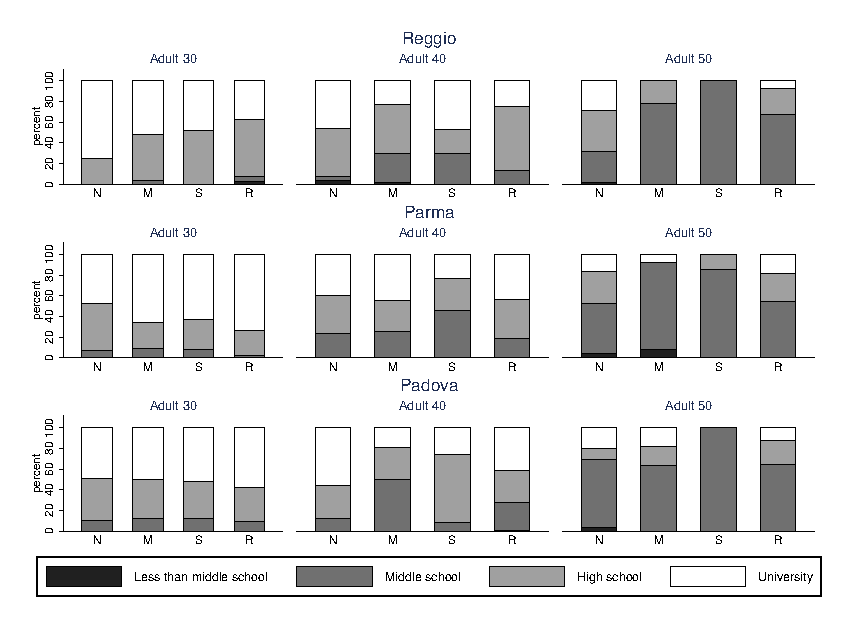
\includegraphics[scale=1.2]{../../Output/image/bar_momEdu}
	\caption{Mother's educational attainment by city, cohort and materna type}
	\label{fig:momEdu}
	\footnotetext{Note:  \textbf{(1)} Definiteion of bar labels: N = Not attended; M = Municipal; S = State; R = Religious. \textbf{(2)} Each bar presents the distribution of mothers' educational attainment for individuals in each city-cohort-materna type combination. }
	\end{minipage}
\end{figure}

\begin{figure}[!htb]
	\begin{minipage}{1\textwidth}
	\centering
	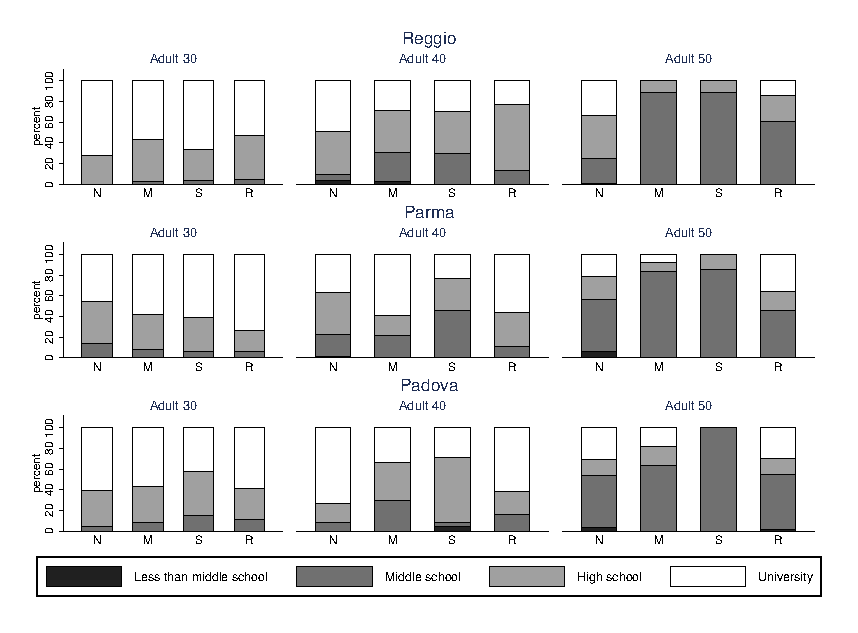
\includegraphics[scale=1.2]{../../Output/image/bar_dadEdu}
	\caption{Father's education attainment by city, cohort and materna type}
	\label{fig:dadEdu}
	\footnotetext{Note:  \textbf{(1)} Definition of bar labels: N = Not attended; M = Municipal; S = State; R = Religious. \textbf{(2)} Each bar presents the distribution of fathers' educational attainment for individuals in each city-cohort-materna type combination. }
	\end{minipage}
\end{figure}

\begin{figure}[!htb]
	\begin{minipage}{.9\textwidth}
	\centering
	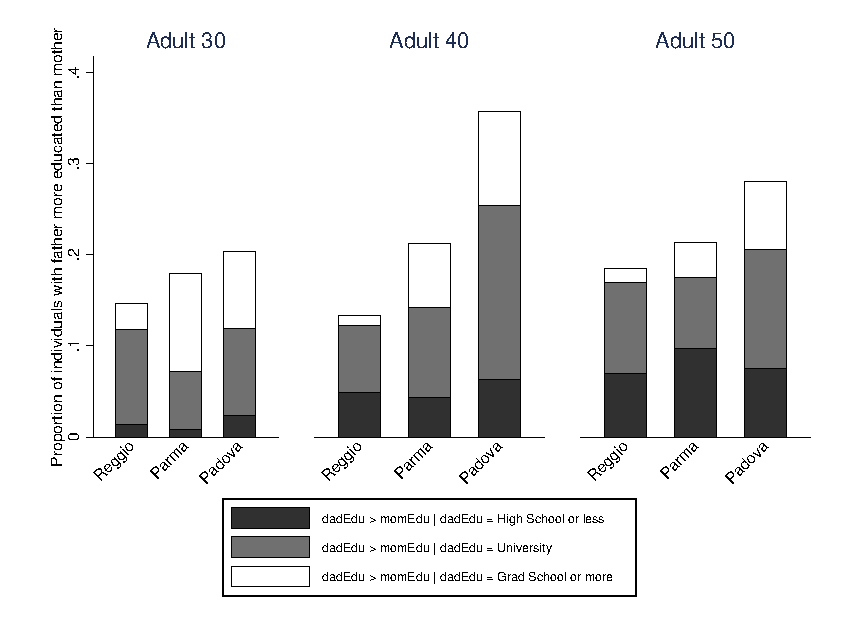
\includegraphics[scale=1]{../../Output/image/bar_parentsEduCompare}
	\caption{Proportion of individuals with fathers who are more educated than mothers by city and cohort}
	\label{fig:parentsEdu}
	\footnotetext{\noindent Note: Each column represents the proportion of individuals within each city-cohort combination whose fathers were more educated than their mothers.}
	\end{minipage}
\end{figure}



\clearpage

%\bibliography{heckman}
%\bibliographystyle{chicago}

\end{document}
